\section{Model Structure}\label{model.str}
The model aims to capture heterosexual HIV transmission among the Swati population aged 15--49.
The model stratifies the modelled population along four dimensions:
two sexes~($s$), four activity groups~($i$), six HIV states~($h$), and five cascade states~($c$),
summarized in Table~\ref{tab:model.dims} and Figure~\ref{fig:model}.
In total, $2 \times 4 \times (1 + 5 \times 5) = 208$ states are modelled.
Two additional ``dimensions'' help organize:
four partnership types ($p$), and two types of sex acts ($a$).
\begin{table}
  \centering
  \caption{Overview of model dimensions and stratifications}
  \label{tab:model.dims}
  \begin{tabular}{lccl}
  \toprule
  Dimension                  & \multicolumn{2}{c}{Index} & Strata \\
  \midrule
  \textbf{Sex}               & ($s$) & 1 & Heterosexual Women    \\
                             &       & 2 & Heterosexual Men      \\[1ex]
  \textbf{Activity group}    & ($i$) & 1 & Lowest Activity       \\
                             &       & 2 & Medium Activity       \\
                             &       & 3 & Lower Risk Sex Work   \\
                             &       & 4 & Higher Risk Sex Work  \\[1ex]
  \textbf{HIV status}        & ($h$) & 1 & Susceptible           \\
                             &       & 2 & Acute HIV             \\
                             &       & 3 & CD4 $>$ 500           \\
                             &       & 4 & 350 $<$ CD4 $<$ 500   \\
                             &       & 5 & 200 $<$ CD4 $<$ 350   \\
                             &       & 6 & CD4 $<$ 200 (AIDS)    \\[1ex]
  \textbf{ART cascade}       & ($c$) & 1 & Undiagnosed           \\
                             &       & 2 & Diagnosed             \\
                             &       & 3 & On ART                \\
                             &       & 4 & Virally Suppressed    \\
                             &       & 5 & Unlinked from Care    \\[1ex] % TODO: implement this change in code
  \textbf{Partnership types} & ($p$) & 1 & Main / Spousal        \\
                             &       & 2 & Casual                \\
                             &       & 3 & Occasional Sex Work   \\
                             &       & 4 & Regular Sex Work      \\[1ex]
  \textbf{Sex act types}     & ($a$) & 1 & Vaginal               \\
                             &       & 2 & Anal                  \\
  \bottomrule
\end{tabular}
  \floatfoot{\centering See footnote \ref{foot:code.note} regarding indices in the code.}
\end{table}
\par
Sexual activity groups were defined to reflect
persistent differences in HIV incidence and prevalence
\cite{SDHS2006,Bicego2013,Justman2016,SHIMS2}
--- reflecting acquisition and/or onward transmission risk ---
as well as common stratifications in the available data,
and epidemiologically relevant sub-populations.
The lowest sexual activity group ($i=1$) comprises
individuals who had 0-1 sexual partners in the past 12 months (p12m),
but did not engage in sex work.
The medium activity group ($i=2$) similarly comprises
individuals who had 2+ sexual partners in p12m
but did not engage in formal sex work.
The highest two activity groups among women ($i=3,4$) comprise
lower and higher risk FSW (see \sref{model.par.fsw} for more details), and
the highest two activity groups among men ($i=3,4$) likewise comprise
lower and higher risk clients of FSW.
% TODO: Watts2010 re pimps, etc.?
\par
Four types of sexual partnerships are modelled,
with different levels of condom use and expected durations:
long-term/spousal partnerships ($p=1$, lowest condom use, 14--19 years);
short-term partnerships ($p=2$, medium condom use, 3--18 months);
one-off new/occasional sex work partnerships ($p=3$, highest condom use, 1 sex act);
and regular sex work partnerships ($p=4$, medium condom use, 2--24 months).
Figure~\ref{fig:model.risk} illustrates
the modelled activity groups and possible partnership types between them.
\begin{figure}
  \begin{subfigure}{\linewidth}
    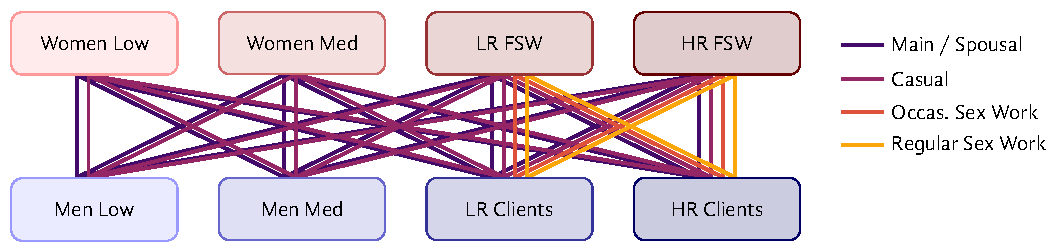
\includegraphics[scale=.8]{model.risk}
    \caption{Activity groups and partnership types}
    \label{fig:model.risk}
  \end{subfigure}
  \begin{subfigure}{\linewidth}
    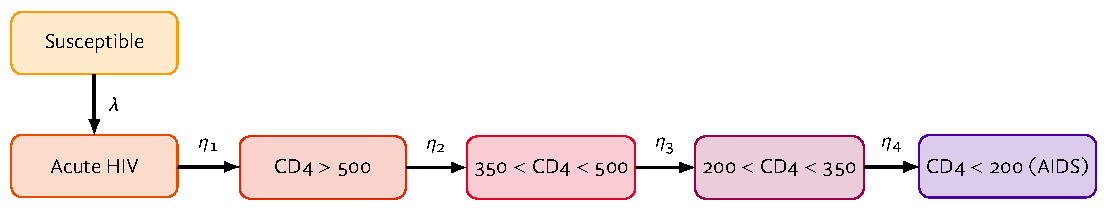
\includegraphics[scale=.8]{model.hiv}
    \caption{HIV states}
    \label{fig:model.hiv}
  \end{subfigure}
  \begin{subfigure}{\linewidth}
    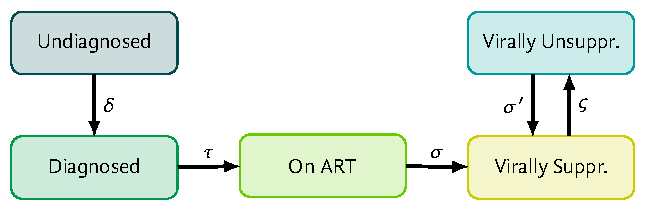
\includegraphics[scale=.8]{model.cascade}
    \caption{ART cascade states}
    \label{fig:model.cascade}
  \end{subfigure}
  \caption{Model structure and transitions}
  \label{fig:model}
  \floatfoot{\ffpops;
    CD4: CD4+ T-cell count per mm\tsup{3};
    Not shown: turnover amongst activity groups in \sfref{fig:model.risk}.}
\end{figure}
\par
HIV infection is stratified into
acute-HIV and stages defined by CD4 count (Figure~\ref{fig:model.hiv})
to reflect changes in mortality~\cite{Mangal2017},
historical ART eligibility~\cite{EswMOH2006,EswMOH2010,EswMOH2015,EswMOH2018},
and, with CD4 as a proxy for viral load, infectiousness~\cite{Boily2009}.
The modelled ART cascade (Figure~\ref{fig:model.cascade})
includes the major steps associated with the ``90-90-90'' targets,
plus a generic ``virally un-suppressed'' state reflecting any combination of
treatment failure, discontinuation, or loss to follow-up after achieving viral suppression.
Loss to follow-up prior to viral suppression is not explicitly modelled,
but subsumed into the rates of ART initiation and viral suppression.
%===================================================================================================
\subsection{Initialization \& Solving}\label{model.init}
The first cases of HIV and AIDS in Eswatini
were diagnosed in 1986 and 1987, respectively \cite{Whiteside2007},
although HIV may have been present several years earlier \cite{Iliffe2005}.
As such, I initialize the model in 1980 with no HIV,
and simulate introduction of HIV at a random year between 1980 and 1985 (uniform prior).
HIV introduction is modelled as
exogenous infection of 0.01\% (\ttilde\,24) individuals in the model,%
\footnote{No further import/export of HIV to/from Eswatini is considered thereafter in the model.
  HIV transmission between Eswatini and neighbouring countries,
  including South Africa and Mozambique,
  has likely continued throughout the epidemic
  due to labour migration and other factors \cite{Iliffe2005}.
  However, I assume that such transmissions have low overall influence on epidemic dynamics.}
  % TODO: discuss possible effects?
distributed across activity groups in proportion to their size, comprising:
% TODO: maybe among highest activity instead?
5\% acute HIV ($h=2$), 65\% with \cdf{500}{} ($h=3$) and 30\% with \cdf{350}{500} ($h=4$),
all undiagnosed ($c=1$).%
\footnote{In compartmental models, the numbers of individuals in each state (compartment)
  need not be whole numbers.}
The population size of EmaSwati aged 15--49 in 1980
was defined as 243,000 from \cite{WorldBank}.
